\section{Introduction}
\label{sec:introduction}


\paragraph{} AC Power is the most commonly used type of electricity, having gained popularity over DC during the latter half of the 19th century. However, many equipments require DC for it's operation, 
specifically devices that use batteries, such as computers or cellphones. Therefore, it is necessary to convert the AC Power obtained either by an alternator (as in the case of a car) or the power grid, to DC.
This process is achieved trough the use of a Rectifier or AC/DC Converter. (In the case of Portugal and most of Europe the power grid runs on 230 V / 50 Hz.)

\paragraph{} The objective of this laboratory assignmente is to model the AC/DC Converter, shown im Figure~\ref{fig:cir}. This circuit is made up of:

\begin{itemize}
	\item Transformer: the element of the circuit responsible for converting AC to DC Power.
	\item Envelope Detector: which "smothens" the original pulsed DC signal.
	\item Voltage Regulator: which reduces the voltage, keeping it close to the 12V target.
\end{itemize}

\paragraph{} In this lab, the Theoretical Analysis is done in Section \ref{sec:analysis}, the Simulation Analysis in Section \ref{sec:simulation}, the results are compared in Section \ref{sec:comparison}. The
Conclusion is presented in Section \ref{sec:conclusion}.

\begin{figure}[h] \centering
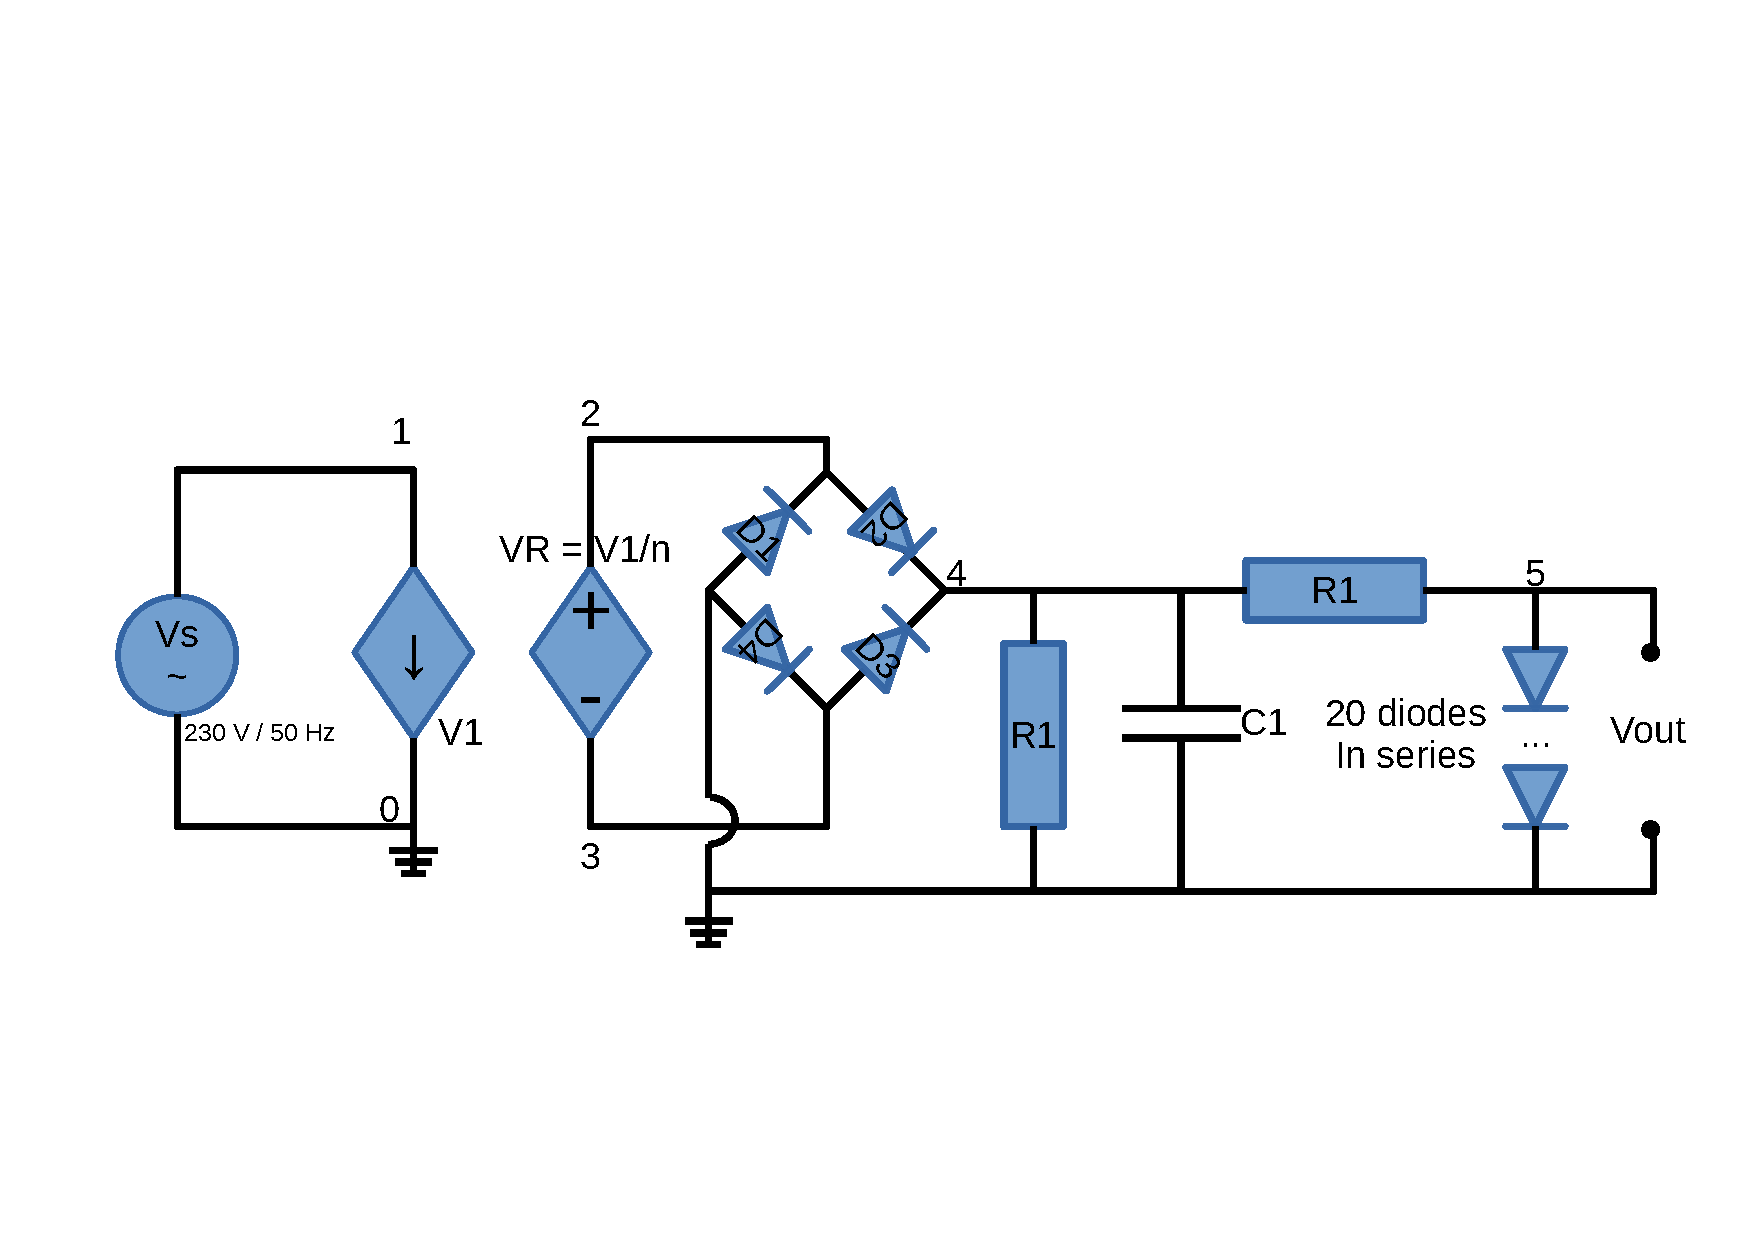
\includegraphics[width=0.7\linewidth]{./cir.pdf}
\caption{The AC/DC converter on which this report is based}
\label{fig:cir}
\end{figure}

\clearpage
